\documentclass[10pt,oneside,american]{amsart}
\usepackage[T1]{fontenc}
\usepackage[latin9]{inputenc}
\setcounter{secnumdepth}{2}
\setcounter{tocdepth}{2}
\usepackage{amstext}
\usepackage{amsthm}
\usepackage{amssymb}
\usepackage{graphicx}

\makeatletter
%%%%%%%%%%%%%%%%%%%%%%%%%%%%%% Textclass specific LaTeX commands.
\numberwithin{equation}{section}
\numberwithin{figure}{section}
  \theoremstyle{plain}
  \newtheorem{thm}{\protect\theoremname}[section]
  \theoremstyle{definition}
  \newtheorem{defn}[thm]{\protect\definitionname}
  \theoremstyle{remark}
  \newtheorem{rem}[thm]{\protect\remarkname}
  \theoremstyle{plain}
  \newtheorem{prop}[thm]{\protect\propositionname}
  \theoremstyle{definition}
  \newtheorem{example}[thm]{\protect\examplename}
  \theoremstyle{plain}
  \newtheorem{lemma}[thm]{Lemma}
  \theoremstyle{plain}
  \newtheorem{conj}[thm]{Conjecture}

%%%%%%%%%%%%%%%%%%%%%%%%%%%%%% User specified LaTeX commands.
\DeclareMathOperator{\sech}{sech}
\DeclareMathOperator{\diag}{diag}
\DeclareMathOperator{\Tr}{tr}
\newcommand{\SPD}{\operatorname{SPD}}

\makeatother

\usepackage{babel}
\providecommand{\definitionname}{Definition}
\providecommand{\examplename}{Example}
\providecommand{\propositionname}{Proposition}
\providecommand{\remarkname}{Remark}
\providecommand{\theoremname}{Theorem}

\begin{document}

\title{Definition and Calculation of Zonal Polynomials}

\author{Lin Jiu and Christoph Koutschan}
\begin{abstract}
In this report, we summarize different definitions of zonal polynomials
involving statistics, differential geometry, representation theory
and combinatorics. A manual of a package for calculating zonal polynomials
is also introduced.
\end{abstract}

\maketitle

\section{Introduction}

In the project proposal \cite[pp.~8]{Proposal}, G.(goal)~2 aims
at hypergeometric function with matrix argument, defined as follows.
\begin{defn}
Given an $m\times m$ symmetric, positive-definite matrix $Y$, the
hypergeometric function with matrix argument is defined as 
\begin{equation}
_{p}F_{q}\left(\genfrac{}{}{0pt}{}{a_{1},\ldots,a_{p}}{b_{1},\ldots,b_{q}}\bigg|Y\right):=\sum_{n=0}^{\infty}\sum_{\lambda\in\mathcal{P}_{n}}\frac{\left(a_{1}\right)_{\lambda}\cdots\left(a_{p}\right)_{\lambda}}{\left(b_{1}\right)_{\lambda}\cdots\left(b_{q}\right)_{\lambda}}\cdot\frac{\mathcal{C}_{\lambda}\left(Y\right)}{n!},\label{eq:MatrixpFq}
\end{equation}
where 
\begin{itemize}
\item $\mathcal{P}_{n}$ is the set of all integer partitions of $n$, where
every partition $\lambda\in\mathcal{P}_{n}$ is defined to be a tuple
$\lambda=\left(\lambda_{1},\ldots,\lambda_{k}\right)$ such that 
\[
\lambda_{1}\geq\lambda_{2}\geq\cdots\geq\lambda_{k}>0
\]
and 
\[
\lambda_{1}+\cdots+\lambda_{k}=n;
\]
\item the Pochhammer symbol, for positive integer $m$, $\left(a\right)_{m}:=a\left(a+1\right)\cdots\left(a+m-1\right)$
is applied to define
\[
\left(a\right)_{\lambda}=\left(a\right)_{\left(\lambda_{1},\dots,\lambda_{k}\right)}:=\prod_{i=1}^{k}\left(a-\frac{i-1}{2}\right)_{\lambda_{i}};
\]
\item and finally $\mathcal{C}_{\lambda}(Y)$ denotes the zonal polynomial
of $Y$, indexed by a partition $\lambda$, which is a symmetric polynomial
of degree $n$, in the eigenvalues $y_{1},\ldots,y_{m}$ of $Y$,
satisfying 
\begin{equation}
\sum_{\lambda\in\mathcal{P}_{n}}\mathcal{C}_{\lambda}\left(Y\right)=\left(\Tr Y\right)^{n}=\left(y_{1}+\cdots+y_{m}\right)^{n}.\label{eq:TrZonal}
\end{equation}
\end{itemize}
\end{defn}
Hashiguchi et.~al \cite{1F1} study the case $p=q=1$, using the holonomic
gradient method \cite[pp.~4--6]{Proposal}. Comparing to the usual
hypergeometric function
\[
_{p}F_{q}\left(\genfrac{}{}{0pt}{}{a_{1},\ldots,a_{p}}{b_{1},\ldots,b_{q}}\bigg|z\right):=\sum_{n=0}^{\infty}\frac{\left(a_{1}\right)_{n}\cdots\left(a_{p}\right)_{n}}{\left(b_{1}\right)_{n}\cdots\left(b_{q}\right)_{n}}\cdot\frac{z^{n}}{n!},
\]
we see that the key is the zonal polynomial $\mathcal{C}_{\lambda}(Y)$,
which inspires this report. Definitions will be presented in Section
\ref{sec:DEFS} and a short manual on a \texttt{Sage} package we implemented
for calculation of $\mathcal{C}_{\lambda}(Y)$ follows
in Section \ref{sec:Package}.

\section{\label{sec:DEFS}Definitions of zonal polynomials}

We shall summarize four different definitions of zonal polynomials
involving statistics, differential geometry, representation theory
and combinatorics. Namely each subsection will present one aspect. 

First of all, we need an important linear space.
\begin{defn}
Let $V_{n}$ be the space of symmetric homogeneous polynomials of
degree $n$ in the variables $y_{1},\ldots,y_{m}$ including the zero polynomial.
Namely, if $f\in V_{n}$, we have 
\begin{itemize}
\item $\deg f=n$ or $f\equiv0$;
\item if $\deg f=n$, then $f$ is symmetric and homogeneous in $y_{1},\ldots,y_{m}$.
\end{itemize}
Moreover, any polynomial $f\in V_{n}$ can also be viewed as a polynomial
in the eigenvalues of $m\times m$ symmetric, positive-definite matrices.
Denote the space of $m\times m$ symmetric, positive-definite matrices
as $\SPD(m)$. 
\end{defn}

\subsection{Definition involving the Wishart distribution}
\begin{defn}
Define the elementary symmetric polynomial \cite[pp.~12, eq.~9]{Takemura}
\[
u_{r}(x_{1},\ldots,x_{m}):=\underset{i_{1}<\cdots<i_{r}}{\sum}x_{i_{1}}\cdots x_{i_{r}}.
\]
Then, for $\lambda=\left(\lambda_{1},\ldots,\lambda_{l}\right)\in\mathcal{P}_{n}$,
the polynomials \cite[pp.~12, eq.~10]{Takemura}
\[
\mathcal{U}_{\lambda}:=u_{1}^{\lambda_{1}-\lambda_{2}}u_{2}^{\lambda_{2}-\lambda_{3}}\cdots u_{l-1}^{\lambda_{l-1}-\lambda_{l}}u_{l}^{\lambda_{l}}
\]
\cite[pp.~13]{Takemura} form a basis for $V_{n}$.
\end{defn}
\begin{rem}
Obviously, 
\[
\deg\mathcal{U}_{\lambda}=\left(\lambda_{1}-\lambda_{2}\right)+2\left(\lambda_{2}-\lambda_{3}\right)+\cdots+l\lambda_{l}=\lambda_{1}+\cdots+\lambda_{l}=n.
\]
Further associate a lexicographical order to $\mathcal{P}_{n}$ \cite[pp.~9, eq.~7]{Takemura}:
for $p=\left(p_{1},\ldots,p_{j}\right),q=\left(q_{1},\ldots,q_{l}\right)\in\mathcal{P}_{n}$,
\[
p>q\Leftrightarrow p_{1}=q_{1},\cdots p_{k-1}=q_{k-1},p_{k}>q_{k}\text{ for some }k.
\]
Then, we could write the basis formed by the $\mathcal{U}_{\lambda}$
as a column vector:
\[
\mathcal{U}:=\left(\mathcal{U}_{\left(n\right)},\mathcal{U}_{\left(n-1,1\right)},\ldots,\mathcal{U}_{\left(1,\ldots,1\right)}\right)^{T}.
\]
\end{rem}
Since this section presents a definition of $\mathcal{C}_{\lambda}(Y)$
related to the Wishart distribution, we shall first define it, as follows.
\begin{defn}
Let $X_{\nu\times m}$ be such that each row is independently drawn
from an $m$-variate normal distribution of mean $0$ and covariance
matrix $V$, namely, 
\[
  \left(x_{i}^{1},\ldots,x_{i}^{m}\right)\sim\mathcal{N}_{m}(0,V)
  \qquad (1\leq i\leq\nu).
\]
Then, we say $S:=X^{T}X$ has the Wishart distribution, denoted by
\[
S=X^{T}X\sim W_{m}(V,\nu),
\]
where $\nu$ is called the degree of freedom.
\end{defn}
\begin{rem}
Recall that in the $1$-dimensional case if $Z_{1},\ldots,Z_{k}\sim\mathcal{N}(0,1)$
are independent Gaussian distributed, then $Q:=Z_{1}+\cdots+Z_{k}\sim\chi_{k}^{2}$.
In other words, the sum of independent Gaussian distributions is chi-square
distributed. The Wishart distribution can be viewed as a multi-dimensional
generalization of the chi-square distribution.
\end{rem}
Define the linear transform \cite[Lem.~2, pp.~19]{Takemura} $\tau_{\nu}\colon V_{n}\longrightarrow V_{n}$,
for $Y\in \SPD(m)$, 
\[
  \left(\tau_{\nu}(\mathcal{U}_{\lambda})\right)\left(Y\right) :=
  \mathbb{E}_{W}\left[\mathcal{U}_{\lambda}(YW)\right]\text{ for }W\sim W(I_m,\nu).
\]
As $\mathcal{U}$ forms a basis of $V_{n}$, $\tau_{\nu}(\mathcal{U}):=\left(\tau_{\nu}(\mathcal{U}_{\left(n\right)}),\tau_{\nu}(\mathcal{U}_{\left(n-1,1\right)}),\ldots,\tau_{\nu}(\mathcal{U}_{\left(1,\ldots,1\right)})\right)^{T}$
must be a linear combination of $\mathcal{U}$ \cite[eq.~19, pp.~22]{Takemura},
denoted by 
\[
\tau_{\nu}(\mathcal{U})=T_{\nu}\mathcal{U}.
\]
Properties of $T_{\nu}$ guarantee that \cite[Lem.~4, pp.~22]{Takemura}
\[
T_{\nu}=\Xi^{-1}\Lambda_{\nu}\Xi,
\]
for some nonsingular upper triangular matrix $\Xi$, which is uniquely
determined up to a (possibly different) multiplicative constant for
each row, and 
\[
\Lambda_{\nu}=\diag\left(2^{n}\overset{k}{\underset{i=1}{\prod}}\left(\frac{\nu+1-i}{2}\right)_{\lambda_{i}},\lambda=\left(\lambda_{1},\ldots,\lambda_{k}\right)\in\mathcal{P}_{n}\right).
\]
Now, we can define zonal polynomials.
\begin{defn}
The zonal polynomial $\mathcal{Y}_{\lambda}$, for a partition $\lambda\in\mathcal{P}_{n}$,
is defined by a vector form
\[
\mathcal{Y}=\left(\begin{matrix}\mathcal{Y}_{\left(n\right)}\\
\mathcal{Y}_{\left(n-1,1\right)}\\
\vdots\\
\mathcal{Y}_{\left(1,\ldots,1\right)}
\end{matrix}\right)=\Xi\,\mathcal{U}=\Xi\left(\begin{matrix}\mathcal{U}_{\left(n\right)}\\
\mathcal{U}_{\left(n-1,1\right)}\\
\vdots\\
\mathcal{U}_{\left(1,\ldots,1\right)}
\end{matrix}\right),
\]
and $\mathcal{C}_{\lambda}(Y)=d_{\lambda}\mathcal{Y}_{\lambda}(Y)$,
where the constants $d_\lambda$ are given by
\[
  d_{\lambda}=\frac{\underset{i<j}{\prod}\left(2\lambda_{i}-2\lambda_{j}-i+j\right)}{\overset{k}{\underset{i=1}{\prod}}\left(2\lambda_{i}+k-i\right)!}
  \cdot\frac{2^{n}n!}{\left(2n\right)!}.
\]
\end{defn}

\subsection{Definition in differential geometry}

We first recall the Laplace-Beltrami operator on Riemannian manifolds.
\begin{defn}
On a Riemannian manifold $\left(M,g\right)$, the Laplace-Beltrami
operator on $f\in C^{\infty}(M)$ is given by 
\[
\Delta f:=\left(\mathrm{div}\bullet\mathrm{grad}\right)f=\sum_{i=1}^{n}\frac{1}{\sqrt{G}}\partial_{k}\left(g^{ik}\sqrt{G}\partial_{i}f\right),
\]
where $n=\dim M$, $\left(g_{ij}\right)_{n\times n}$ is the metric
matrix and $G:=\det\left(g_{ij}\right)$. 
\end{defn}
\begin{rem}
When $M=\mathbb{R}^{n}$ and $\left(g_{ij}\right)=I_{n}$, the identity
matrix, then 
\[
\Delta f=\sum_{i=1}^{n}\frac{\partial^{2}f}{\partial x_{i}^{2}}.
\]
Namely, the Laplace-Beltrami operator is the generalization of the Laplace
operator on $\mathbb{R}^{n}$. 
\end{rem}
\begin{prop}
Given $X\in \SPD(m)$, James \cite[eq.~3.12, pp.~1712]{James1} derived
that the Laplace-Beltrami operator is given by
\[
\Delta=\sum_{i=1}^{m}\left(y_{i}^{2}\frac{\partial^{2}}{\partial y_{i}^{2}}-\frac{m-3}{2}y_{i}\frac{\partial}{\partial y_{i}}+\sum_{j=1,j\neq i}^{m}\frac{y_{i}^{2}}{y_{i}-y_{j}}\frac{\partial}{\partial y_{i}}\right),
\]
where $X=HYH^{T}$, for $H\in O(n)$ and $Y=\diag(y_{1},\ldots,y_{n})$. 
\end{prop}
\begin{rem}
The second term in the parentheses is, up to the constant $\frac{m-3}{2}$,
the Euler's operator $\overset{m}{\underset{i=1}{\sum}}y_{i}\frac{\partial}{\partial y_{i}}$,
which has all symmetric, homogeneous polynomials as its eigenfunctions.
Thus, when considering any eigenfunction of the Laplace-Beltrami operator~$\Delta$,
this term can be eliminated.
\end{rem}
\begin{defn}
The zonal polynomials $\mathcal{C}_{\lambda}(y_{1},\ldots,y_{m})$
are eigenfunctions of $\Delta_{Y}$, defined by
\[
  \Delta_{Y}:=\sum_{i=1}^{m}\left(y_{i}^{2}\frac{\partial^{2}}{\partial y_{i}^{2}}+\sum_{j=1,j\neq i}^{m}\frac{y_{i}^{2}}{y_{i}-y_{j}}\frac{\partial}{\partial y_{i}}\right).
\]
In particular
\[
  \Delta_{Y}\mathcal{C}_{\lambda}(Y)=\left(\rho_{\lambda}+(m-1)n\right)\mathcal{C}_{\lambda}(Y)
  \qquad (n=\lambda_1+\dots+\lambda_k),
\]
where
\begin{equation}
  \rho_{\lambda}:=\sum_{i=1}^{k}\lambda_{i}\left(\lambda_{i}-i\right).\label{eq:RHO}
\end{equation}
\end{defn}

\subsection{Definition through representation theory}

Consider the general linear group $G=\mathrm{GL}(m)$ on
$V_{n}$. Define a representation 
\begin{eqnarray*}
g\in\mathrm{GL}(m):V_{n} & \rightarrow & V_{n}\\
\varphi\left(Y\right) & \mapsto & \varphi\left(g^{-1}Y\left(g^{-1}\right)^{T}\right)
\end{eqnarray*}
As a representation, the linear space can be decomposed into invariant
subspaces \cite[pp.~611]{Representation}
\[
V_{n}=\bigoplus_{\lambda\in\mathcal{P}_{n}}V_{\lambda}.
\]

\begin{defn}
For given $Y\in \SPD(m)$ and a partition $\lambda\in\mathcal{P}_{n}$,
the projection
\begin{equation}
\left(\Tr Y\right)^{n}\bigg|_{V_{\lambda}}=\mathcal{C}_{\lambda}(Y)\label{eq:projection}
\end{equation}
defines the zonal polynomials.
\end{defn}
\begin{rem}
\eqref{eq:projection} confirms \eqref{eq:TrZonal}. 
\end{rem}

\subsection{A short remark on Macdonald, Jack and zonal polynomials}

Special case of Macdonald polynomial gives Jack polynomials $J_{\lambda}^{\left(\alpha\right)}$,
which when $\alpha=2$ gives zonal polynomials. 

\section{\label{sec:Package}Sage package for the calculation of zonal polynomials}

Although there are more than one ways to define the zonal polynomial $\mathcal{C}_{\lambda}(Y)$,
in practice, none of these definition gives an algorithm or formula
to directly compute $\mathcal{C}_{\lambda}(Y)$. Now, we
follow the steps by Muirhead \cite{Muirhead} to build up a package for the
calculation of $\mathcal{C}_{\lambda}(Y)$.
\begin{defn}
For $\lambda=\left(\lambda_{1},\ldots,\lambda_{l}\right)\in\mathcal{P}_{n}$,
define the \emph{monomial symmetric function} as 
\begin{equation}
\mathcal{M}_{\lambda}(y_{1},\ldots,y_{m})=\sum_{\genfrac{}{}{0pt}{}{i_{1},\ldots,i_{l}}{\text{distinct terms}}}y_{i_{1}}^{\lambda_{1}}\cdots y_{i_{l}}^{\lambda_{l}}=y_{1}^{\lambda_{1}}\cdots y_{l}^{\lambda_{l}}+\text{symmetric terms}.\label{eq:MZonal}
\end{equation}
\end{defn}
\begin{example}
Let $Y$ be an $m\times m$ symmetric matrix with eigenvalues $y_{1},\ldots,y_{m}$:
\begin{enumerate}
\item 
\[
\mathcal{M}_{\left(1\right)}(Y)=y_{1}+\cdots+y_{m};
\]
\item 
\[
\mathcal{M}_{\left(2\right)}(Y)=y_{1}^{2}+\cdots+y_{m}^{2};
\]
\item \label{enu:ILessThanJ}
\[
\mathcal{M}_{\left(1,1\right)}(Y)=\underset{i<j}{\sum}y_{i}y_{j};
\]
\item \label{enu:IANDJ}
\[
\mathcal{M}_{\left(2,1\right)}(Y)=\underset{i,j}{\sum}y_{i}^{2}y_{j}.
\]
\end{enumerate}
Here we see the last two functions have the same length of partitions
but different sum ranges, due to the fact that $y_{1}y_{2}$ and $y_{2}y_{1}$
are the same while $y_{1}^{2}y_{2}$ and $y_{2}^{2}y_{1}$ are different. 
\end{example}
\begin{rem}
An explicit expression of $M_{\lambda}(Y)$ is given by
\cite[pp.~11, eq.~6]{Takemura}:
\begin{equation}
\mathcal{M}_{\left(1^{m_{1}}2^{m_{2}}\cdots\right)}\left(Y\right)=\left(\prod_{i=1}^{h}\frac{1}{m_{i}!}\right)\sum_{i_{1},\ldots,i_{l}}y_{i_{1}}^{\lambda_{1}}\cdots y_{i_{l}}^{\lambda_{l}}.\label{eq:MZonalComputation}
\end{equation}
\end{rem}
\begin{thm}
A general result by James \cite{James1} shows that
\begin{equation}
C_{\kappa}(Y)=\sum_{\lambda\leq\kappa}c_{\kappa,\lambda}M_{\lambda}(Y),\label{eq:CInTermsOfM}
\end{equation}
 for some constants $c_{\kappa,\lambda}$. (see also \cite[pp.~234, eq.~13]{Muirhead}).
\end{thm}
Note that $M_\lambda(Y)$ is defined to be zero whenever there are fewer variables
than parts in the partition~$\lambda$. It follows that $C_{\kappa}(Y)=0$ if the
dimension of~$Y$ is smaller than the number of parts of~$\kappa$.
\begin{example}
\label{Tables}The following tables \cite[pp.~238]{Muirhead} show
constants $c_{\kappa,\lambda}$, in the case $n=\left|\kappa\right|=\left|\lambda\right|=2,\ldots5$. 
\begin{itemize}
\item $n=2$
\[
\def\arraystretch{1.3}
\begin{array}{c|cc}
\kappa\backslash\lambda & \left(2\right) & \left(1,1\right)\\ \hline
\left(2\right) & 1 & \frac{2}{3}\\
\left(1,1\right) & 0 & \frac{4}{3}
\end{array}
\]
\item $n=3$
\[
\def\arraystretch{1.3}
\begin{array}{c|ccc}
\kappa\backslash\lambda & \left(3\right) & \left(2,1\right) & \left(1,1,1\right)\\ \hline
\left(3\right) & 1 & \frac{3}{5} & \frac{2}{5}\\
\left(2,1\right) & 0 & \frac{12}{5} & \frac{18}{5}\\
\left(1,1,1\right) & 0 & 0 & 2
\end{array}
\]
\item $n=4$
\[
\def\arraystretch{1.3}
\begin{array}{c|ccccc}
\kappa\backslash\lambda & \left(4\right) & \left(3,1\right) & \left(2,2\right) & \left(2,1,1\right) & \left(1,1,1,1\right)\\ \hline
\left(4\right) & 1 & \frac{4}{7} & \frac{18}{35} & \frac{12}{35} & \frac{8}{35}\\
\left(3,1\right) & 0 & \frac{24}{7} & \frac{16}{7} & \frac{88}{21} & \frac{32}{7}\\
\left(2,2\right) & 0 & 0 & \frac{16}{5} & \frac{32}{15} & \frac{16}{5}\\
\left(2,1,1\right) & 0 & 0 & 0 & \frac{16}{3} & \frac{64}{5}\\
\left(1,1,1,1\right) & 0 & 0 & 0 & 0 & \frac{16}{5}
\end{array}
\]
\item $n=5$
\[
\def\arraystretch{1.3}
\begin{array}{c|ccccccc}
\kappa\backslash\lambda & \left(5\right) & \left(4,1\right) & \left(3,2\right) & \left(3,1,1\right) & \left(2,2,1\right) & \left(2,1,1,1\right) & \left(1,1,1,1,1\right)\\ \hline
\left(5\right) & 1 & \frac{5}{9} & \frac{10}{21} & \frac{20}{63} & \frac{2}{7} & \frac{4}{21} & \frac{8}{63}\\
\left(4,1\right) & 0 & \frac{40}{9} & \frac{8}{3} & \frac{46}{9} & 4 & \frac{14}{3} & \frac{40}{9}\\
\left(3,2\right) & 0 & 0 & \frac{48}{7} & \frac{32}{7} & \frac{176}{21} & \frac{64}{7} & \frac{80}{7}\\
\left(3,1,1\right) & 0 & 0 & 0 & 10 & \frac{20}{3} & \frac{130}{7} & \frac{200}{7}\\
\left(2,2,1\right) & 0 & 0 & 0 & 0 & \frac{32}{3} & 16 & 32\\
\left(2,1,1,1\right) & 0 & 0 & 0 & 0 & 0 & \frac{80}{7} & \frac{800}{21}\\
\left(1,1,1,1,1\right) & 0 & 0 & 0 & 0 & 0 & 0 & \frac{16}{3}
\end{array}
\]
\end{itemize}
\end{example}
\begin{thm}
The constant $c_{\kappa,\lambda}$ satisfies the recurrence \cite[pp.~234, eq.~14]{Muirhead}
\begin{equation}
c_{\kappa,\lambda}=\sum_{\lambda<\mu\leq\kappa}\frac{\left(\lambda_{i}+t\right)-\left(\lambda_{j}-t\right)}{\rho_{\kappa}-\rho_{\lambda}}c_{\kappa,\mu},\label{eq:CRec}
\end{equation}
where for $\lambda=\left(\lambda_{1},\ldots,\lambda_{l}\right)$,
the sum is over all $\mu=\left(\lambda_{1},\ldots,\lambda_{i}+t,\ldots,\lambda_{j}-t,\ldots,\lambda_{l}\right)$
for $t=1,\ldots,\lambda_{j}$ such that by rearranging the tuple~$\mu$
in a descending order, it lies as $\lambda<\mu\leq\kappa$.
\end{thm}
\begin{rem}
Observing \eqref{eq:CRec}, once given initial $c_{\kappa,\kappa}$,
$\forall\lambda<\kappa$, it could compute $c_{\kappa,\lambda}$.
Now, observing tables in Example \ref{Tables} and recall \eqref{eq:TrZonal},
it is easy to see that for each column, the sum is given by a multinomial
coefficient. More concretely, let $\lambda=\left(\lambda_{1},\ldots,\lambda_{l}\right)\in\mathcal{P}_{n}$,
\begin{equation}
  \sum_{\kappa=\lambda}^{\left(n\right)}c_{\kappa,\lambda}=\binom{n}{\lambda_{1},\ldots,\lambda_{l}}.\label{eq:CInitial}
\end{equation}
In particular, $c_{\left(n\right),\left(n\right)}=\binom{n}{n}=1$.
Thus, all constants $c_{\kappa,\lambda}$ are obtained, so is $C_{\lambda}(Y)$. 
\end{rem}

\subsection{Functions}

~\\
~
\noindent \begin{flushleft}
\textbf{Calmi}(\emph{partition)}
\par\end{flushleft}

\noindent \begin{flushleft}
calculate the product of factorials in front of the sum on the right-hand
side of \eqref{eq:MZonalComputation}.
\par\end{flushleft}

\noindent \begin{flushleft}
\rule[0.5ex]{1\columnwidth}{1pt}
\par\end{flushleft}

\noindent \begin{flushleft}
\textbf{MZonal}(\emph{partition},\emph{variables)}
\par\end{flushleft}

\noindent \begin{flushleft}
computes the monomial symmetric function using \eqref{eq:MZonalComputation}.
\par\end{flushleft}

\noindent \begin{flushleft}
\rule[0.5ex]{1\columnwidth}{1pt}
\par\end{flushleft}

\noindent \begin{flushleft}
\textbf{SumVariable}\emph{($\kappa$,$\lambda$)}
\par\end{flushleft}

\noindent \begin{flushleft}
computes the list of $\mu$ appearing in the summation of \eqref{eq:CRec},
according to the paragraph under.
\par\end{flushleft}

\noindent \begin{flushleft}
\rule[0.5ex]{1\columnwidth}{1pt}
\par\end{flushleft}

\noindent \begin{flushleft}
\textbf{RHO}(\emph{partition)}
\par\end{flushleft}

\noindent \begin{flushleft}
computes $\rho_{\lambda}$ from \eqref{eq:RHO}.
\par\end{flushleft}

\noindent \begin{flushleft}
\rule[0.5ex]{1\columnwidth}{1pt}
\par\end{flushleft}

\noindent \begin{flushleft}
\textbf{Coeffi}\emph{(kappa,lambda)}
\par\end{flushleft}

\noindent \begin{flushleft}
computes the constants $c_{\kappa,\lambda}$ through \eqref{eq:CRec}
and \eqref{eq:CInitial}.
\par\end{flushleft}

\noindent \begin{flushleft}
\rule[0.5ex]{1\columnwidth}{1pt}
\par\end{flushleft}

\noindent \begin{flushleft}
\textbf{CZonal}\emph{(partition},\emph{variables)}
\par\end{flushleft}

\noindent \begin{flushleft}
computes the zonal polynomial $C_{\lambda}\left(y_{1},\ldots,y_{m}\right)$
through linear combination \eqref{eq:CInTermsOfM}.
\par\end{flushleft}

\subsection{Examples}
\noindent \begin{flushleft}
In{[}1{]}= \textbf{Coeffi({[}2, 1{]}, {[}1, 1, 1{]})}\\
~\\
Out{[}1{]}=$18/5$\\
~\\
In{[}2{]}= \textbf{MZonal({[}2, 1{]}, {[}a, b, c{]})}\\
~\\
Out{[}2{]}=$a^{2}b+ab^{2}+a^{2}c+b^{2}c+ac^{2}+bc^{2}$\\
~\\
In{[}2{]}= \textbf{CZonal{[}{[}2, 1{]}, {[}a, b, c{]})}\\
~\\
Out{[}2{]}=$\frac{12}{5}\left(a^{2}b+ab^{2}+a^{2}c+b^{2}c+ac^{2}+bc^{2}\right)+\frac{18}{5}abc$
\par\end{flushleft}

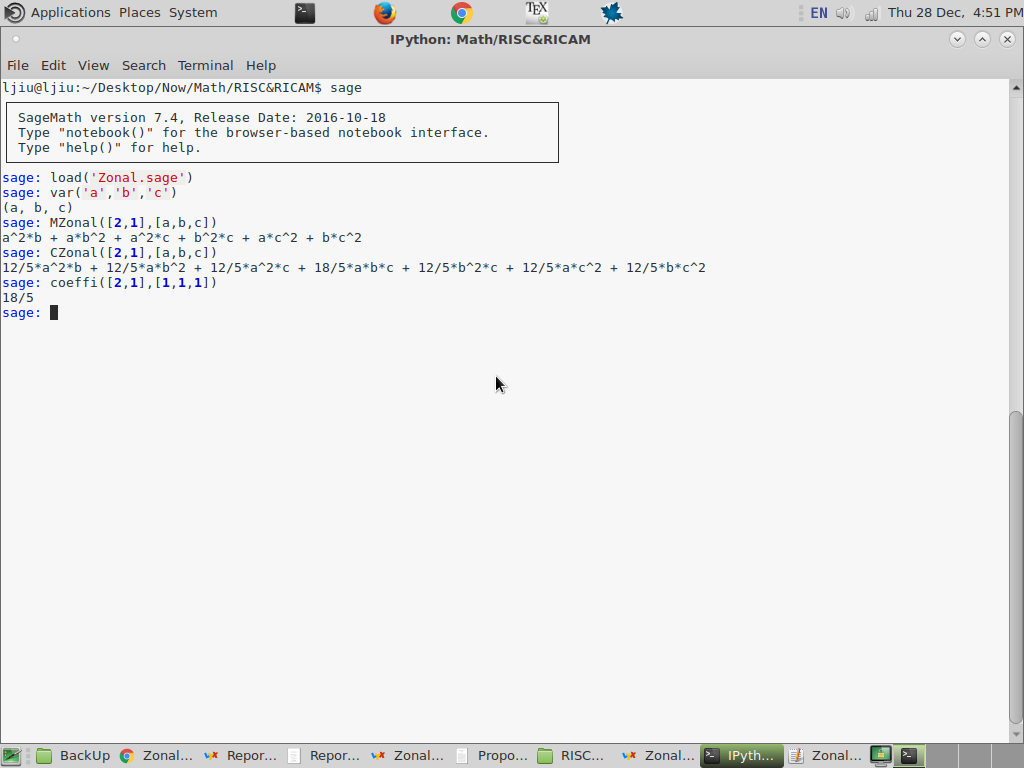
\includegraphics[scale=0.3]{ScreenShot}


\section{Infinite Families of Coefficients $c_{\kappa,\lambda}$}

In this section, we study some infinite families among the coefficients
$c_{\kappa,\lambda}$ of the zonal polynomials~$C_{\kappa}(Y)$. Since we have
seen that $c_{(n),(n)}=1$ for all~$n$ (that corresponds to the upper left
corner of the $c_{\kappa,\lambda}$-matrix), one can ask whether the
``neighboring'' entries also admit a closed form for general~$n$.
Theorem~\ref{thm:fam1} will give an explicit answer for the first few cases.
Before that, we focus on the first row of the $c_{\kappa,\lambda}$-matrix,
i.e., on the coefficients $c_{\kappa,\lambda}$ for which
$\kappa=\left(n\right)$ and $\lambda\leq\kappa$ has two parts.

\begin{thm}\label{thm:row1}
Let $\left(n-m,m\right)$ be a partition of $n$, then
\begin{equation}\label{eq:1to2}
  c_{\left(n\right),\left(n-m,m\right)} =
  %\frac{\left(2m-1\right)!!n\left(n-1\right)\cdots\left(n-m+1\right)}{m!\left(2n-1\right)\left(2n-3\right)\cdots\left(2n-\left(2m-1\right)\right)}
  \binom{n}{m}\cdot\frac{\bigl(\frac12\bigr)_m}{\bigl(n-m+\frac12\bigr)_m}.
\end{equation}
%where for an odd positive integer $a$, $a!!:=a\left(a-2\right)\left(a-4\right)\cdots1$. 
\end{thm}
\begin{proof}
It is obvious that $\rho_{\left(n\right)}=n\left(n-1\right)$ and $\rho_{\left(n-m,m\right)}=\left(n-m\right)\left(n-m-1\right)+m\left(m-2\right)$,
so that 
\[%begin{equation}
  \rho_{\left(n\right)}-\rho_{\left(n-m,m\right)}=m\left(2n-2m+1\right). \label{eq:coeff1to2}
\]%end{equation}
By \eqref{eq:CRec},
\begin{align*}
  c_{\left(n\right),\left(n-m,m\right)}
  &= \sum_{\left(n-m,m\right)<\mu\leq\left(n\right)}\frac{\left(n-m+t\right)-\left(m-t\right)}
    {\rho_{\left(n\right)}-\rho_{\left(n-m,m\right)}}\cdot c_{\left(n\right),\mu} \\
  &= \frac{1}{m\left(2n-2m+1\right)}\sum_{t=1}^{m}\left(n-2m+2t\right)c_{\left(n\right),\mu}.
\end{align*}
Now, we proceed by induction on~$m$. Obviously, $ \rho_{\left(n\right)}-\rho_{\left(n-1,1\right)}=2n-1$. 
Moreover, the only possible $\mu$ satisfying $\left(n-1,1\right)<\mu\leq\left(n\right)$
is $\mu=\left(n\right)$ with $t=1$. Therefore, 
\begin{equation}\label{eq:cnton1}
  c_{\left(n\right),\left(n-1,1\right)}=\frac{\left(n-1+1\right)-\left(1-1\right)}{2n-1}\cdot1=\frac{n}{2n-1}.
\end{equation}
Now, assume \eqref{eq:1to2} holds. We have
\begin{align*}
 & c_{\left(n\right),\left(n-m-1,m+1\right)} = \\
 &= \frac{1}{\left(m+1\right)\left(2\left(n-m\right)-1\right)}\sum_{t=1}^{m+1}\left(n-2m-2+2t\right)c_{\left(n\right),\mu}\\
 &= \frac{1}{\left(m+1\right)\left(2\left(n-m\right)-1\right)}\biggl(\left(n-2m\right)c_{\left(n\right),\left(n-m,m\right)}+\sum_{t=2}^{m+1}\left(n-2m-2+2t\right)c_{\left(n\right),\mu}\biggr)\\
 &= \frac{1}{\left(m+1\right)\left(2\left(n-m\right)-1\right)}\biggl(\left(n-2m\right)c_{\left(n\right),\left(n-m,m\right)}+\sum_{t=1}^{m}\left(n-2m+2t\right)c_{\left(n\right),\mu}\biggr)\\
 &= \frac{c_{\left(n\right),\left(n-m,m\right)}}{\left(m+1\right)\left(2\left(n-m\right)-1\right)}\Bigl(\left(n-2m\right)+m\left(2\left(n-m\right)+1\right)\Bigr) \\
 &= \frac{\left(n-m\right)\left(2m+1\right)}{\left(m+1\right)\left(2\left(n-m\right)-1\right)}\cdot\binom{n}{m}\frac{\bigl(\frac12\bigr)_m}{\bigl(n-m+\frac12\bigr)_m}
 = \binom{n}{m+1}\cdot\frac{\bigl(\frac12\bigr)_{m+1}}{\bigl(n-m-\frac12\bigr)_{m+1}}.
\end{align*}
\end{proof}

\begin{thm}
\label{thm:fam1}
We have
\begin{alignat*}{2}
  c_{(n-1,1),(n-1,1)} &= \frac{2n(n-1)}{2n-1}, &\qquad& (n\geq2) \\
  c_{(n-1,1),(n-2,2)} &= \frac{2n(n-1)(n-2)}{(2n-1)(2n-5)}, && (n\geq4) \\
  c_{(n-2,2),(n-2,2)} &= \frac{2n(n-1)(n-2)(n-3)}{(2n-3)(2n-5)}, &&(n\geq4).
\end{alignat*}
\end{thm}
\begin{proof}
Using \eqref{eq:CInitial} with $\lambda=(n-1,1)$,
\[
  c_{\left(n\right),\left(n-1,1\right)}+c_{\left(n-1,1\right),\left(n-1,1\right)}=\binom{n}{n-1,1}=n,
\]
and \eqref{eq:cnton1} we get
\[
  c_{\left(n-1,1\right),\left(n-1,1\right)}=n-\frac{n}{2n-1}=\frac{2n^{2}-2n}{2n-1}=\frac{2n\left(n-1\right)}{2n-1}.
\]
By applying \eqref{eq:CRec}, we obtain
\begin{align*}
  c_{\left(n-1,1\right),\left(n-2,2\right)}
  &= \frac{\left(n-2+1\right)-\left(2-1\right)}{\rho_{\left(n-1,1\right)}-\rho_{\left(n-2,2\right)}}\cdot c_{(n-1,1),(n-1,1)}\\
  &= \frac{\left(n-2+1\right)-\left(2-1\right)}{\left(n-1\right)n-2n+1-\left(n-2\right)\left(n-3\right)}\cdot\frac{2n\left(n-1\right)}{2n-1}\\
  &= \frac{2n\left(n-1\right)\left(n-2\right)}{\left(2n-1\right)\left(2n-5\right)}.
\end{align*}
Finally, using~\eqref{eq:CInitial} with $\lambda=(n-2,2)$ and
Theorem~\ref{thm:row1}, we get the last coefficient:
\begin{align*}
  c_{\left(n-2,2\right),\left(n-2,2\right)}
  &= \binom{n}{n-2,2}-c_{\left(n\right),\left(n-2,2\right)}-c_{\left(n-1,1\right),\left(n-2,2\right)}\\
  &= \frac{n\left(n-1\right)}{2}-\frac{3n\left(n-1\right)}{2\left(2n-1\right)\left(2n-3\right)}-\frac{2n\left(n-1\right)\left(n-2\right)}{\left(2n-1\right)\left(2n-5\right)}\\
  &= \frac{2n\left(n-1\right)\left(n-2\right)\left(n-3\right)}{\left(2n-3\right)\left(2n-5\right)}.
\end{align*}
\end{proof}

It is clear that we could proceed in this manner and compute more coefficients
$c_{\kappa,\lambda}$ in the upper left corner of the matrix for symbolic~$n$.
Since the corresponding calculations get too tedious to be done by hand, we
employ computer algebra to determine the rational function expressions for a
few more coefficients.  Note that, when $n$ is sufficiently large, the
lexicographically largest elements of $\mathcal{P}_n$ are (in descending
order): %$(n)$, $(n-1,1)$, $(n-2,2)$, $(n-2,1,1)$, $(n-3,3)$, etc.
\[
  (n), \; (n-1,1), \; (n-2,2), \; (n-2,1,1), \; (n-3,3), \; (n-3,2,1), \; \text{etc.}
\]
In Table~\ref{tab:cn1} we give closed forms for the coefficients
$c_{\kappa,\lambda}$ when $\kappa$ and $\lambda$ are taken from these
lexicographically largest partitions, i.e., when both $\kappa$ and $\lambda$
are of the form $(n-m,\pi)$, where $\pi$ is a partition of~$m\in\mathbb{N}$,
but where $n$ is symbolic.  Pictorially speaking, this table represents the
upper left submatrix of the $c_{\kappa,\lambda}$-matrix for large~$n$; more
precisely, for $n\geq6$ since we consider only partitions
$(n),\dots,(n-3,1,1,1)$. We remark that all these formulas have been
rigorously proven by applying \eqref{eq:CRec} and~\eqref{eq:CInitial} for
symbolic~$n$, as it was done in the proof of Theorem~\ref{thm:fam1}. This
symbolic proof strategy is implemented in our Mathematica package.
% TODO: add reference and name of the procedure

\begin{table}
\[
  \def\arraystretch{1.3}
  \begin{array}{c|ccccc}
    \kappa\backslash\lambda &
    (n) & (n-1,1) & (n-2,2) & (n-2,1,1) & (n-3,3) \\ \hline
    \rule{0pt}{14pt} (n) &
    1 & \frac{n}{2 n-1} & \frac{3 (n-1) n}{2 (2 n-3) (2 n-1)} & \frac{(n-1)
      n}{(2 n-3) (2 n-1)} & \frac{5 (n-2) (n-1) n}{2 (2 n-5) (2 n-3) (2 n-1)}
    \\[1ex]
    (n-1,1) &
    0 & \frac{2 (n-1) n}{2 n-1} & \frac{2 (n-2) (n-1) n}{(2 n-5) (2 n-1)} &
    \frac{2 n (2 n^2-6 n+3)}{(2 n-5) (2 n-1)} & \frac{3 (n-3) (n-2)
      (n-1) n}{(2 n-7) (2 n-5) (2 n-1)} \\[1ex]
    (n-2,2) &
    0 & 0 & \frac{2 (n-3) (n-2) (n-1) n}{(2 n-5) (2 n-3)} & \frac{4 (n-3)
      (n-2) (n-1) n}{3 (2 n-5) (2 n-3)} & \frac{2 (n-4) (n-3) (n-2) (n-1)
      n}{(2 n-9) (2 n-5) (2 n-3)} \\[1ex]
    (n-2,1,1) &
    0 & 0 & 0 & \frac{2}{3} (n-2) n & 0 \\[1ex]
    (n-3,3) &
    0 & 0 & 0 & 0 & \frac{4 (n-5) (n-4) (n-3) (n-2) (n-1) n}{3 (2 n-9) (2 n-7) (2 n-5)}
  \end{array}
\]
\[
  \def\arraystretch{1.3}
  \begin{array}{c|ccccc}
    \kappa\backslash\lambda &
    (n-3,2,1) & (n-3,1,1,1) % & (n-4,4) & (n-4,3,1) & (n-4,2,2)
    \\ \hline
    \rule{0pt}{14pt} (n) &
    \frac{3 (n-2) (n-1) n}{2 (2 n-5) (2 n-3) (2 n-1)}
    & \frac{(n-2) (n-1) n}{(2 n-5) (2 n-3) (2 n-1)} 
    % & \frac{35 (n-3) (n-2) (n-1) n}{8 (2 n-7) (2 n-5) (2 n-3) (2 n-1)}
    % & \frac{5 (n-3) (n-2) (n-1) n}{2 (2 n-7) (2 n-5) (2 n-3) (2 n-1)}
    % & \frac{9 (n-3) (n-2) (n-1) n}{4 (2 n-7) (2 n-5) (2 n-3) (2 n-1)}
    \\[1ex]
    (n-1,1) &
    \frac{(n-2) n (5 n^2-20 n+11)}{(2 n-7) (2 n-5) (2 n-1)}
    & \frac{6 (n-2) n (n^2-4 n+2)}{(2 n-7) (2 n-5) (2 n-1)}
    % & \frac{5 (n-4) (n-3) (n-2) (n-1) n}{(2 n-9) (2 n-7) (2 n-5) (2 n-1)}
    % & \frac{(n-3) (n-2) n (8 n^2-40 n+23)}{(2 n-9) (2 n-7) (2 n-5) (2 n-1)}
    % & \frac{6 (n-3) (n-2) n (n^2-5 n+3)}{(2 n-9) (2 n-7) (2 n-5) (2 n-1)}
    \\[1ex]
    (n-2,2) &
    \frac{2 (n-3) (n-1) n (5 n^2-30 n+36)}{3 (2 n-9) (2 n-5) (2 n-3)}
    & \frac{4 (n-3) (n-1) n (n^2-6 n+7)}{(2 n-9) (2 n-5) (2 n-3)}
    % & \frac{3 (n-5) (n-4) (n-3) (n-2) (n-1) n}{(2 n-11) (2 n-9) (2 n-5) (2 n-3)}
    % & \frac{4 (n-4) (n-3) (n-1) n (n^2-7 n+9)}{(2 n-11) (2 n-9) (2 n-5) (2 n-3)}
    % & \frac{2 (n-1) n (11 n^4-154 n^3+761 n^2-1554 n+1098)}{3 (2 n-11) (2 n-9) (2 n-5) (2 n-3)}
    \\[1ex]
    (n-2,1,1) &
    \frac{2 (n-3) (n-2) n}{3 (2 n-7)}
    & \frac{2 (n-2) n (2 n^2-9 n+8)}{(2 n-7) (2 n-3)}
    % & 0
    % & \frac{(n-4) (n-3) (n-2) n}{(2 n-9) (2 n-7)}
    % & \frac{2 (n-4) (n-3) (n-2) n}{3 (2 n-9) (2 n-7)}
    \\[1ex]
    (n-3,3) &
    \frac{4 (n-5) (n-4) (n-3) (n-2) (n-1) n}{5 (2 n-9) (2 n-7) (2 n-5)}
    & \frac{8 (n-5) (n-4) (n-3) (n-2) (n-1) n}{15 (2 n-9) (2 n-7) (2 n-5)}
    % & \frac{4 (n-6) (n-5) (n-4) (n-3) (n-2) (n-1) n}{3 (2 n-13) (2 n-9) (2 n-7) (2 n-5)}
    % & \frac{4 (n-5) (n-4) (n-2) (n-1) n (8 n^2-72 n+135)}{15 (2 n-13) (2 n-9) (2 n-7) (2 n-5)}
    % & \frac{8 (n-5) (n-4) (n-2) (n-1) n (n^2-9 n+17)}{5 (2 n-13) (2 n-9) (2 n-7) (2 n-5)}
    \\[1ex]
    (n-3,2,1) &
    \frac{4 (n-4) (n-3) (n-1) n}{5 (2 n-7)}
    & \frac{6 (n-4) (n-3) (n-1) n}{5 (2 n-7)}
    % & 0
    % & \frac{4 (n-5) (n-4) (n-3) (n-1) n}{5 (2 n-11) (2 n-7)}
    % & \frac{4 (n-3) (n-1) n (2 n^2-18 n+39)}{5 (2 n-11) (2 n-7)}
    \\[1ex]
    (n-3,1,1,1) &
    0 & \frac{2 (n-3) (n-2) (n-1) n}{3 (2 n-3)}
    % & 0 & 0 & 0
    \\[1ex]
    (n-4,4) &
    0 & 0
    % & \frac{2 (n-7) (n-6) (n-5) (n-4) (n-3) (n-2) (n-1) n}{3 (2 n-13) (2 n-11) (2 n-9) (2 n-7)}
    % & \frac{8 (n-7) (n-6) (n-5) (n-4) (n-3) (n-2) (n-1) n}{21 (2 n-13) (2 n-11) (2 n-9) (2 n-7)}
    % & \frac{12 (n-7) (n-6) (n-5) (n-4) (n-3) (n-2) (n-1) n}{35 (2 n-13) (2 n-11) (2 n-9) (2 n-7)}
    %% \\[1ex]
    %% (n-4,3,1) &
    %% 0 & 0
    %% % & 0
    %% % & \frac{4 (n-6) (n-5) (n-4) (n-2) (n-1) n}{7 (2 n-11) (2 n-9)}
    %% % & \frac{8 (n-6) (n-5) (n-4) (n-2) (n-1) n}{21 (2 n-11) (2 n-9)}
    %% \\[1ex]
    %% (n-4,2,2) &
    %% 0 & 0
    %% % & 0 & 0 & \frac{2}{15} (n-5) (n-2) (n-1) n
  \end{array}
\]
\caption{Coefficients $c_{\kappa,\lambda}$ for some of the lexicographically
  largest partitions of~$n$; the lower table continues the upper one to the
  right.}
\label{tab:cn1}
\end{table}
\begin{example}
For example, for $n=23$ we obtain the coefficient $c_{(21,2),(21,1,1)}$ by
looking at the entry in Table~\ref{tab:cn1} in row $(n-2,2)$ and column
$(n-2,1,1)$:
\[
  c_{(21,2),(21,1,1)} = \frac{4 (n-3) (n-2) (n-1) n}{3 (2 n-5) (2 n-3)} \Big|_{n\to23}
  = \frac{4 \cdot 20 \cdot 21 \cdot 22 \cdot 23}{3 \cdot 41 \cdot 43}
  = \frac{283360}{1763}.
\]
\end{example}

The next families we study are located in the ``lower right corner'' of
$c_{\kappa,\lambda}$-matrix. In this case both $\kappa$ and $\lambda$ are of
the form $(2^m,1^{n-2m})$, i.e., a sequence of $m$ times the part~$2$ and
$n-2m$ times the part~$1$. Note that for $m=0,1,2,\dots$ we obtain the
lexicographically smallest partitions of~$n$ (in increasing order).  In
contrast to Theorem~\ref{thm:fam1} it is not straightforward to derive
formulas for general~$n$ by means of Equations \eqref{eq:CRec}
and~\eqref{eq:CInitial}. Instead, we compute the first few values of these
sequences, say up to $n=30$, and then guess a closed form expression. The
first few results are displayed in Table~\ref{tab:cn2}.

More precisely, we first applied the \texttt{Guess} package~\cite{Guess} to
find a plausible candidate for a linear recurrence with polynomial
coefficients (in all considered instances this recurrence was of first order,
which easily allowed for a closed form solution). Then, after observing that
all expressions obtained this way were of the form $2^n\cdot r(n)$ where
$r(n)$ is some rational function in~$n$, we refined our ansatz to only search
for expressions of this form: divide the $n$-th sequence entry by $2^n$ and
then perform polynomial interpolation and rational reconstruction.

\begin{table}
\[
  \def\arraystretch{1.3}
  \begin{array}{c|ccc}
    \kappa\backslash\lambda
    % & (2^6,1^{n-12}) & (2^5,1^{n-10})
    & (2^4,1^{n-8}) & (2^3,1^{n-6}) & (2^2,1^{n-4})
    % & (2,1^{n-2}) & (1^n)
    \\ \hline
    %% (2^6,1^{n-12})
    %% & \frac{1}{315} 2^{n-4} (n-10) (n-9) (n-2) (n-1) n
    %% & \frac{1}{315} 2^{n-4} (n-11) (n-10)^2 (n-2) (n-1) n
    %% & \frac{1}{315} 2^{n-5} (n-11) (n-10)^2 (n-9) (n-2) (n-1) n
    %% & \frac{1}{945} 2^{n-5} (n-11) (n-10)^2 (n-9) (n-6) (n-2) (n-1) n
    %% & \frac{1}{945} 2^{n-7} (n-11) (n-10)^2 (n-9) (n-5) (n-4) (n-2) (n-1) n
    %% & ?
    %% & ?
    %% \\[1ex]
    %% (2^5,1^{n-10})
    %% & 0
    %% & \frac{1}{45} 2^{n-4} (n-8) (n-7) (n-1) n
    %% & \frac{1}{45} 2^{n-4} (n-9) (n-8)^2 (n-1) n
    %% & \frac{1}{45} 2^{n-5} (n-9) (n-8)^2 (n-7) (n-1) n
    %% & \frac{1}{135} 2^{n-5} (n-9) (n-8)^2 (n-7) (n-4) (n-1) n
    %% & \frac{1}{135} 2^{n-7} (n-9) (n-8)^2 (n-7) (n-3) (n-2) (n-1) n
    %% & \frac{1}{675} 2^{n-7} (n-9) (n-8)^2 (n-7) (n-2) (n-1)^2 n^2
    %% \\[1ex]
    \rule{0pt}{14pt}
    (2^4,1^{n-8})
    % & 0 & 0
    & \frac{2^{n-3} (n-6) (n-5) n}{15}
    & \frac{2^{n-3} (n-7) (n-6)^2 n}{15}
    & \frac{2^{n-4} (n-7) (n-6)^2 (n-5) n}{15}
    % & \frac{2^{n-4} (n-7) (n-6)^2 (n-5) (n-2) n}{45}
    % & \frac{2^{n-6} (n-7) (n-6)^2 (n-5) (n-1) n^2}{45}
    \\[1ex]
    (2^3,1^{n-6})
    % & 0 & 0
    & 0
    & \frac{2^{n-3} (n-4) (n-3)}{3}
    & \frac{2^{n-3} (n-5) (n-4)^2}{3}
    % & \frac{2^{n-4} (n-5) (n-4)^2 (n-3)}{3}
    % & \frac{2^{n-4} (n-5) (n-4)^2 (n-3) n}{9}
    \\[1ex]
    (2^2,1^{n-4})
    % & 0 & 0
    & 0 & 0
    & \frac{2^{n-1} (n-2) (n-1)}{3 (n+1)}
    % & \frac{2^{n-1} (n-3) (n-2)^2}{3 (n+1)}
    % & \frac{2^{n-2} (n-3) (n-2)^2 (n-1)}{3 (n+1)}
    \\[1ex]
    (2,1^{n-2})
    % & 0 & 0
    & 0 & 0 & 0
    % & \frac{2^{n-1} n}{n+2}
    % & \frac{2^{n-1} (n-1) n^2}{(n+1) (n+2)}
    \\[1ex]
    (1^n)
    % & 0 & 0
    & 0 & 0 & 0
    % & 0 & \frac{2^n}{n+1}
\end{array}
\]
\[
  \def\arraystretch{1.3}
  \begin{array}{c|cc}
    \kappa\backslash\lambda
    & (2,1^{n-2}) & (1^n) \\ \hline
    \rule{0pt}{14pt}
    (2^4,1^{n-8})
    & \frac{2^{n-4} (n-7) (n-6)^2 (n-5) (n-2) n}{45}
    & \frac{2^{n-6} (n-7) (n-6)^2 (n-5) (n-1) n^2}{45}
    \\[1ex]
    (2^3,1^{n-6})
    & \frac{2^{n-4} (n-5) (n-4)^2 (n-3)}{3}
    & \frac{2^{n-4} (n-5) (n-4)^2 (n-3) n}{9}
    \\[1ex]
    (2^2,1^{n-4})
    & \frac{2^{n-1} (n-3) (n-2)^2}{3 (n+1)}
    & \frac{2^{n-2} (n-3) (n-2)^2 (n-1)}{3 (n+1)}
    \\[1ex]
    (2,1^{n-2})
    & \frac{2^{n-1} n}{n+2}
    & \frac{2^{n-1} (n-1) n^2}{(n+1) (n+2)}
    \\[1ex]
    (1^n)
    & 0 & \frac{2^n}{n+1}
\end{array}
\]
\caption{Coefficients $c_{\kappa,\lambda}$ for some of the lexicographically
  smallest partitions of~$n$; the lower table continues the upper one to the
  right.}
\label{tab:cn2}
\end{table}

Muirhead~\cite[Lemma~7.2.3]{Muirhead} gives a necessary condition for some
coefficients $c_{\kappa,\lambda}$ to be zero, but without proof. We recall his
result here and give a simple proof of it.
\begin{lemma}\label{lem:zero1}
  Let $n\in\mathbb{N}$ and $\kappa,\lambda$ be partitions of~$n$ with $p$ and
  $q$ parts, respectively. If $p>q$, i.e., if $\kappa$ has more parts
  than~$\lambda$, then $c_{\kappa,\lambda}=0$.
\end{lemma}
\begin{proof}
  From the definition of zonal polynomials it follows
  \begin{align*}
    0 = C_{\kappa}(y_1,\dots,y_{p-1}) &=
    \sum_{\lambda\leq\kappa} c_{\kappa,\lambda} M_{\lambda}(y_1,\dots,y_{p-1}) \\
    &= \!\!\!\!\!\sum_{\genfrac{}{}{0pt}{}{\lambda\leq\kappa}{\operatorname{parts}(\lambda)<p}}\!\!\!\!\!
      c_{\kappa,\lambda} \underbrace{M_{\lambda}(y_1,\dots,y_{p-1})}_{\neq0} \quad +
    \sum_{\genfrac{}{}{0pt}{}{\lambda\leq\kappa}{\operatorname{parts}(\lambda)\geq p}}\!\!\!\!\!
      c_{\kappa,\lambda} \underbrace{M_{\lambda}(y_1,\dots,y_{p-1})}_{=0}
  \end{align*}
  from which it becomes apparent that all coefficients $c_{\kappa,\lambda}$
  for which $\lambda$ has fewer parts than $p=\operatorname{parts}(\kappa)$
  must be zero.
\end{proof}

While Lemma~\ref{lem:zero1} only gives a necessary condition under which
$c_{\kappa,\lambda}$ is zero, we would like to obtain a full characterization,
i.e., a necessary and sufficient condition for $c_{\kappa,\lambda}=0$. For
example, we have $c_{(8,2,2),(7,4,1)} = 0$ although both partitions have the
same length.
\begin{lemma}\label{lem:zero2}
  Let $n\in\mathbb{N}$ and let $\kappa$ and $\lambda$ be two partitions of~$n$
  with $\kappa\geq\lambda$ in lexicographic order. If there exists
  $p\in\mathbb{N}$ such that
  \begin{equation}\label{eq:prop}
    \sum_{i=1}^p (\kappa_i - \lambda_i) < 0
  \end{equation}
  (where the partitions are filled with zeros as necessary), then
  $c_{\kappa,\lambda}=0$.
\end{lemma}
\begin{proof}
  We first want to show that, under the assumption~\eqref{eq:prop},
  $\sum_{i=1}^p(\kappa_i-\mu_i)<0$ holds for all $\mu$ of the form
  $\mu=(\dots,\lambda_r+t,\dots,\lambda_s-t,\dots)$, $1\leq t\leq \lambda_s$,
  after reordering the parts. Assume that this reordering requires us
  to move the part $\lambda_r+t$ to the $k$-th position ($k\leq r$) and
  the part $\lambda_s-t$ to the $\ell$-th position ($\ell\geq s$). Then
  the partition~$\mu$ has the following form:
  \[
    (\lambda_1,\dots,\lambda_{k-1},\lambda_r+t,\lambda_k,\dots,
    \lambda_{r-1},\lambda_{r+1},\dots,\lambda_{s-1},\lambda_{s+1},\dots,
    \lambda_{\ell},\lambda_s-t,\lambda_{\ell+1},\dots).
  \]
  Then we have
  \[
    \sum_{i=1}^p \mu_i =
    \begin{cases}
      \sum_{i=1}^p \lambda_i & \text{if } p<k \\
      \sum_{i=1}^{p-1} \lambda_i + \lambda_r+t & \text{if } k\leq p<r \\
      \sum_{i=1}^p \lambda_i + t & \text{if } r\leq p<s \\
      \sum_{i=1}^{s-1} \lambda_i + t + \sum_{i=s+1}^{p+1}\lambda_i & \text{if } s\leq p<\ell \\
      \sum_{i=1}^p \lambda_i & \text{if } p\geq\ell.
    \end{cases}
  \]
  In each of these cases, we have $\sum_{i=1}^p \mu_i \geq \sum_{i=1}^p
  \lambda_i$.  For the first, third, and fifth case, this is immediately
  obvious. For the second and fourth case, it is true because
  $\lambda_r+t\geq\lambda_p$ and $\lambda_{p+1}\geq\lambda_s-t$, respectively.

  Note that the $\mu$'s in~\eqref{eq:CRec} are exactly of the above form.
  Hence, if $\kappa$ and $\lambda$ satisfy~\eqref{eq:prop}, then
  $c_{\kappa,\lambda}$ is a linear combination of $c_{\kappa,\mu}$'s with the
  same property. In order to conclude the proof by induction, we have to
  investigate the two possible base cases:
  \begin{enumerate}
  \item We arrive at a $c_{\kappa,\lambda}$ for which $\lambda$ has fewer
    parts than~$\kappa$ (note that the operation
    $(\dots,\lambda_r+t,\dots,\lambda_s-t,\dots)$ weakly decreases the number
    of parts). Then by Lemma~\ref{lem:zero1} we have $c_{\kappa,\lambda}=0$.
  \item We arrive at a $c_{\kappa,\lambda}$ such that no suitable $\mu$
    between $\lambda$ and $\kappa$ exists.  Also in this case we get
    $c_{\kappa,\lambda}=0$ since the sum in~\eqref{eq:CRec} is empty.
  \end{enumerate}
\end{proof}

\begin{conj}
  The converse of Lemma~\eqref{lem:zero2} holds, i.e., $c_{\kappa,\lambda}=0$
  only if \eqref{eq:prop} holds. (We have tested this conjecture up to
  $n=22$.)
\end{conj}

\begin{example}
  For $\kappa=(8,2,2)$ and $\lambda=(7,4,1)$ we verify that the second
  partial sum of their differences, i.e. $j=2$, is negative:
  $(8-7)+(2-4)=-1$, and hence $c_{\kappa,\lambda}$ must be zero.
\end{example}


\section{Partitions with two parts}

Now we concentrate on the coefficients $c_{\kappa,\lambda}$ when both $\kappa$
and $\lambda$ have at most two parts. Then, on the one hand, the
partitions~$\mu$ that appear in the recursive formula~\eqref{eq:CRec} have
also at most two parts, by the way how they are constructed from~$\lambda$. On
the other hand, when we use Equation~\eqref{eq:CInitial} to compute
$c_{\lambda,\lambda}$, only those coefficients $c_{\kappa,\lambda}$ contribute
for which $\kappa$ has at most two parts; this is a direct consequence of
Lemma~\ref{lem:zero1}.  We conclude that for the computation of
$c_{\kappa,\lambda}$ we do not need any $c_{\kappa',\lambda'}$ with $\kappa'$
or $\lambda'$ having more than two parts.

\noindent
Throughout this section we write
\[
  \kappa=(a,a-b) \quad\text{and}\quad \lambda=(a-d,a-b+d)
\]
for nonnegative integers $a,b,d$.  The condition $b<a$ ensures that $\kappa$
is a proper partition and the condition $d\leq\frac{b}{2}$ ensures that the
parts of $\lambda$ are in the correct order. In Theorem~\ref{thm:cf2} we
present a closed form of the coefficients $c_{\kappa,\lambda}$ under these
assumptions. We start our investigation by specializing
Equations~\eqref{eq:CRec} and~\eqref{eq:CInitial} to partitions with two
parts.

First of all, it is easy to compute that 
\begin{align*}
  \rho_{\kappa} &= a(a-1) + (a-b)(a-b-2), \\
  \rho_{\lambda} &= (a-d)(a-d-1) + (a-b+d)(a-b+d-2),
\end{align*}
so that
\[
  \rho_{\kappa}-\rho_{\lambda} = d\cdot(2b-2d+1).
\]
Then, the recurrence~\eqref{eq:CRec} can be written as follows, by noting that
$\lambda$ has only two parts,
\begin{align}\label{eq:rec2}
  c_{\kappa,\lambda} = c_{(a,a-b),(a-d,a-b+d)} &=
  \sum_{\lambda<\mu\leq\kappa}\frac{(a-d+t)-(a-b+d-t)}{\rho_{\kappa}-\rho_{\lambda}} c_{\kappa,\mu} \notag \\
  &= \sum_{t=1}^d\frac{b-2d+2t}{d\,(2b-2d+1)}c_{(a,a-b),(a-d+t,a-b+d-t)} \\
  &= \sum_{j=0}^{d-1} \frac{b-2j}{d\,(2b-2d+1)}c_{(a,a-b),(a-j,a-b+j)}. \notag
\end{align}

\begin{example}\label{ex:twoparts}
We begin with some concrete examples.  For $\kappa=(a,a-b)$ and
$\lambda=\left(a-d,a-b+d\right)$ for $d=1,2,3$, we obtain
\begin{align*}
  c_{\left(a,a-b\right),\left(a-1,a-b+1\right)} &= \frac{b}{2b-1}\,c_{\left(a,a-b\right),\left(a,a-b\right)}, \\
  c_{\left(a,a-b\right),\left(a-2,a-b+2\right)} &=
    \frac{1}{4b-6}\Bigl((b-2)\,c_{(a,a-b),(a-1,a-b-1)}+b\,c_{(a,a-b),(a,a-b)}\Bigr) \\
  &= \frac{c_{\left(a,a-b\right),\left(a,a-b\right)}}{4b-6}\left(\frac{\left(b-2\right)b}{2b-1}+b\right) \\
  &= \frac{3b\left(b-1\right)}{2\left(2b-1\right)\left(2b-3\right)}\,c_{(a,a-b),(a,a-b)}, \\
  c_{\left(a,a-b\right),\left(a-3,a-b+3\right)} &=
    \frac{1}{3\left(2b-5\right)}\Bigl(\left(b-4\right)c_{(a,a-b),(a-2,a-b+2)} \\
    &\qquad +\left(b-2\right)c_{(a,a-b),(a-1,a-b+1)}+b\, c_{(a,a-b),(a,a-b)}\Bigr)\\
  &= \frac{c_{\left(a,a-b\right),\left(a,a-b\right)}}{3\left(2b-5\right)}
    \left(\left(b-4\right)\frac{3b\left(b-1\right)}{2\left(2b-1\right)\left(2b-3\right)}+\frac{3b\left(b-1\right)}{2b-1}\right)\\
  &= \frac{5b\left(b-1\right)\left(b-2\right)}{2\left(2b-1\right)\left(2b-3\right)\left(2b-5\right)}\,c_{(a,a-b),(a,a-b)}.
\end{align*}
%% \item For $\lambda=\left(a-4,a-b+4\right)$, 
%% \begin{align*}
%% c_{\left(a,a-b\right),\left(a-4,a-b+4\right)} & =\frac{1}{4\left(2b-7\right)}\left[\left(b-6\right)c_{\left(a,a-b\right),\left(a-3,a-b+3\right)}+c_{\left(a,a-b\right),\left(a-3,a-b+3\right)}\cdot3\left(2b-5\right)\right]\\
%%  & =\frac{7\left(b-3\right)}{4\left(2b-7\right)}c_{\left(a,a-b\right),\left(a-3,a-b+3\right)}\\
%%  & =\frac{7\cdot5b\left(b-1\right)\left(b-2\right)\left(b-3\right)}{4\cdot2\left(2b-1\right)\left(2b-3\right)\left(2b-5\right)\left(2b-7\right)}c_{\left(a,a-b\right),\left(a,a-b\right)}\\
%%  & =\frac{7\cdot5\cdot3b\left(b-1\right)\left(b-2\right)\left(b-3\right)}{4\cdot3\cdot2\left(2b-1\right)\left(2b-3\right)\left(2b-5\right)\left(2b-7\right)}c_{\left(a,a-b\right),\left(a,a-b\right)}
%% \end{align*}
\end{example}

\begin{prop}\label{prop:p2row}
  Given two partitions $\kappa=(a,a-b)$ and $\lambda=(a-d,a-b+d)$ of the positive integer $n=2a-b$,
  with $0\leq b<a$ and $0\leq d\leq\frac{b}{2}$, then
  \begin{equation}\label{eq:2PartRec}
    c_{\kappa,\lambda} = c_{(a,a-b),(a-d,a-b+d)} =
    \binom{b}{d}\,\frac{\bigl(\frac12\bigr)_{\!d}}{\bigl(b-d+\frac12\bigr)_{\!d}} \cdot c_{(a,a-b),(a,a-b)}.
  \end{equation}
\end{prop}
\begin{proof}
  Note that this result is a direct generalization of Theorem~\ref{thm:row1},
  and hence the same inductive argument could be applied. Instead, we
  illustrate a different proof strategy, using symbolic summation. Because of
  the recursive definition of the coefficients $c_{\kappa,\lambda}$,
  demonstrated in Example~\ref{ex:twoparts}, it suffices to show that the
  asserted expression satisfies the recurrence~\eqref{eq:rec2}. This means, we
  have to prove the following identity:
  \begin{equation}\label{eq:sumid}
    \binom{b}{d}\,\frac{\bigl(\frac12\bigr)_{\!d}}{\bigl(b-d+\frac12\bigr)_{\!d}} =
    \sum_{j=0}^{d-1} \binom{b}{j}\,\frac{(b-2j)\,\bigl(\frac12\bigr)_{\!j}}{d\,(2b-2d+1)\,\bigl(b-j+\frac12\bigr)_{\!j}}.
  \end{equation}
  Using special-purpose computer algebra packages, such as the
  HolonomicFunctions package~\cite{HolonomicFunctions}, we find that the
  expression in the sum, denote it by $f(j)$, is Gosper-summable. More
  precisely, we find a function
  \[
    g(j) = \frac{j\,(2b-2j+1)}{b-2j} \cdot f(j) =
    \binom{b}{j}\frac{j\,(2b-2j+1) \bigl(\frac12\bigr)_{\!j}}{d\,(2b-2d+1)\,\bigl(b-j+\frac12\bigr)_{\!j}}
  \]
  with the property $g(j+1)-g(j)=f(j)$ (the latter can be easily
  verified). By telescoping, and by noting that $g(0)=0$, we obtain
  the value of the right-hand side of~\eqref{eq:sumid}:
  \[
    g(d) = \binom{b}{d}\cdot\frac{\bigl(\frac12\bigr)_{\!d}}{\bigl(b-d+\frac12\bigr)_{\!d}}
  \]
  which matches exactly the left-hand side of~\eqref{eq:sumid}.
\end{proof}



\begin{thm}\label{thm:cf2}
  Let $a,b,d\in\mathbb{N}$ with $0\leq b<a$ and $0\leq d\leq\frac{b}{2}$.
  Then we have
  \[
    c_{(a,a-b),(a-d,a-b+d)} = 
    \frac{(2a-b)! \, \bigl(b+\frac12\bigr) \, \bigl(\frac12\bigr)_{\!d}}
         {d! \, (a-b)! \, (b-d)! \, \bigl(b-d+\frac12\bigr)_{\!a-b+d+1}}.
  \]
\end{thm}
\begin{proof}
  We first show that the asserted expression is compatible with the result of
  Proposition~\ref{prop:p2row}: indeed, computing the quotient
  \begin{align*}
    \frac{c_{(a,a-b),(a-d,a-b+d)}}{c_{(a,a-b),(a,a-b)}} &=
    \frac{(2a-b)! \, \bigl(b+\frac12\bigr) \, \bigl(\frac12\bigr)_{\!d} \cdot
      (a-b)! \, b! \, \bigl(b+\frac12\bigr)_{\!a-b+1}}
      {d! \, (a-b)! \, (b-d)! \, \bigl(b-d+\frac12\bigr)_{\!a-b+d+1} \cdot
        (2a-b)! \, \bigl(b+\frac12\bigr)} \\
    &= \frac{b! \, \bigl(\frac12\bigr)_{\!d} \, \bigl(b+\frac12\bigr)_{\!a-b+1}}
      {d! \, (b-d)! \, \bigl(b-d+\frac12\bigr)_{\!a-b+d+1}}
    = \binom{b}{d}\,\frac{\bigl(\frac12\bigr)_{\!d}}{\bigl(b-d+\frac12\bigr)_{\!d}},
  \end{align*}
  we see that this is the case. It remains to prove that the asserted
  expression is correct in the case $d=0$, i.e., for $\kappa=\lambda$.  For
  this purpose, we employ the recursion~\eqref{eq:CInitial}, specialized to
  partitions with two parts:
  \begin{equation}\label{eq:CInitial2}
    \sum_{d=0}^{a-b} c_{(a+d,a-b-d),(a,a-b)} = \binom{2a-b}{a}.
  \end{equation}
  By dividing both sides with the binomial coefficient of the right-hand side,
  and by inserting the asserted closed form (after the change of variables
  $a\to a+d$ and $b\to b+2d$), we are left with the summation identity
  \begin{equation}\label{eq:sumid2}
    \sum_{d=0}^{a-b}
    \frac{a! \, (a-b)! \, \bigl(b+2d+\frac{1}{2}\bigr) \, \bigl(\frac{1}{2}\bigr)_{\!d}}
         {d! \, (a-b-d)! \, (b+d)! \, \bigl(b+d+\frac12\bigr)_{\!a-b+1}} = 1.
  \end{equation}
  Taking into account the recursive definition of the coefficients
  $c_{\kappa,\lambda}$, the (inductive) proof is completed by
  verifying~\eqref{eq:sumid2}.

  For this purpose, we denote by $f(a,b,d)$ the expression inside the
  sum~\eqref{eq:sumid2} and construct two WZ pairs, i.e., two functions
  \begin{align*}
    g_1(d) &= \frac{-2d(b+d)}{(a-b-d+1)(2b+4d+1)}\cdot f(a,b,d) \\
    &= -\frac{a! \, (a-b)! \, \bigl(\frac12\bigr)_{\!d}}{(d-1)! \, (b+d-1)! \, (a-b-d+1)! \, \bigl(b+d+\frac12\bigr)_{\!a-b+1}}, \\
    g_2(d) &= \frac{d(2a+2d+1)}{(a-b)(2b+4d+1)} \cdot f(a,b,d) \\
    &= \frac{a! \, (a-b-1)! \, \bigl(\frac12\bigr)_{\!d}}{(d-1)! \, (b+d)! \, (a-b-d)! \, \bigl(b+d+\frac12\bigr)_{\!a-b}},
  \end{align*}
  such that the following identities hold (they can be verified by routine
  calculations):
  \begin{align}
    f(a+1,b,d)-f(a,b,d) &= g_1(d+1) - g_1(d), \label{eq:WZ1} \\
    f(a,b+1,d)-f(a,b,d) &= g_2(d+1) - g_2(d). \label{eq:WZ2}
  \end{align}
  Now we sum \eqref{eq:WZ1} for $d=0,\dots,a-b$ and obtain
  \[
    \sum_{d=0}^{a-b}\bigl(f(a+1,b,d)-f(a,b,d)\bigr) = g_1(a-b+1) - g_1(a,0)
  \]
  or, equivalently:
  \[
    \sum_{d=0}^{a-b+1}f(a+1,b,d) - \sum_{d=0}^{a-b}f(a,b,d) = g_1(a-b+1) - g_1(a,0) + f(a+1,b,a-b+1).
  \]
  A straightforward calculation shows that the left-hand side equals~$0$,
  thereby showing that the sum $\sum_{d=0}^{a-b}f(a,b,d)$ is independent
  of~$a$. Summing over \eqref{eq:WZ2}, followed by a similar calculation,
  shows that the sum does not depend on~$b$ as well. Therefore, the sum
  in~\eqref{eq:sumid2} is constant, and by setting $a=b=0$ one immediately
  sees that this constant is~$1$.
\end{proof}

% TODO remark case b=a
\begin{rem}
  By setting $b=a$ in Theorem~\ref{thm:cf2} and by interpreting $(a,0)$ as the
  partition~$(a)$, we recover Theorem~\ref{thm:row1}:
  \[
    c_{(a),(a-d,d)} = 
    \frac{(a)! \, \bigl(a+\frac12\bigr) \, \bigl(\frac12\bigr)_{\!d}}
         {d! \, (a-d)! \, \bigl(a-d+\frac12\bigr)_{\!d+1}} =
    \binom{a}{d} \, \frac{\bigl(\frac12\bigr)_{\!d}}{\bigl(a-d+\frac12\bigr)_{\!d}}.
  \]
\end{rem}



\subsection{Not sure where this should go}

Now, from \cite[eq.~18, p.~237]{Muirhead} we see when $y_{1}=y_{2}=1$,
\[
\mathcal{C}_{\kappa}\left(1,1\right)=2^{2N}N!\left(2\right)_{n}\left(0\right)_{m}\frac{2\left(n-m\right)-1+2}{\left(2n+1\right)!\left(2m\right)!}=2^{2n}\frac{N!\left(n+1\right)!\left(m-1\right)!\left(2s+1\right)}{\left(2n+1\right)!\left(2m\right)!}.
\]
\begin{itemize}
\item When $n$ and $m$ have different parities, i.e., for all $\lambda=\left(n-d,m+d\right)\leq\kappa$,
$M_{\lambda}\left(1,1\right)=2$. Therefore, we have 
\[
2^{2n}\frac{N!\left(n+1\right)!\left(m-1\right)!\left(2s+1\right)}{\left(2n+1\right)!\left(2m\right)!}=2c_{\left(n,m\right),\left(n,m\right)}\sum_{d=1}^{\frac{s-1}{2}}\frac{\left(2d-1\right)!!s\left(s-1\right)\cdots\left(s-d+1\right)}{d!\left(2s-1\right)\left(2s-3\right)\cdots\left(2s-2d+1\right)},
\]
i.e, 
\[
c_{\left(n,m\right),\left(n,m\right)}=\frac{\left(2n+1\right)!\left(2m\right)!}{2^{2n-1}N!\left(n+1\right)!\left(m-1\right)!\left(2s+1\right)}\sum_{d=1}^{\frac{s-1}{2}}\frac{\left(2d-1\right)!!s\left(s-1\right)\cdots\left(s-d+1\right)}{d!\left(2s-1\right)\left(2s-3\right)\cdots\left(2s-2d+1\right)}.
\]
\item When $n$ and $m$ have the same parity, i.e., $s=n-m$ is even, for
all $\lambda=\left(n-d,m+d\right)\leq\kappa$, $M_{\lambda}\left(1,1\right)=2$,
except that $M_{\left(n-\frac{s}{2},m+\frac{s}{2}\right)}\left(1,1\right)=1$.
Thus, we have 
\begin{align*}
 & 2^{2n}\frac{N!\left(n+1\right)!\left(m-1\right)!\left(2s+1\right)}{\left(2n+1\right)!\left(2m\right)!},\\
 & =c_{\left(n,m\right),\left(n,m\right)}\left[2\sum_{d=1}^{\frac{s}{2}-1}\frac{\left(2d-1\right)!!s\left(s-1\right)\cdots\left(s-d+1\right)}{d!\left(2s-1\right)\left(2s-3\right)\cdots\left(2s-2d+1\right)}+\frac{\left(s-1\right)!!s\left(s-1\right)\cdots\left(\frac{s}{2}+1\right)}{\left(\frac{s}{2}\right)!\left(2s-1\right)\left(2s-3\right)\cdots\left(s+1\right)}\right],
\end{align*}
which also gives $c_{(n,m),(n,m)}$. 
\end{itemize}





\begin{thebibliography}{1}
\bibitem{1F1}H.~Hashiguchi, Y.~Numata, N.~Takayama, and A.~Takemura.
The holonomic gradient method for the distribution function of the
largest root of a Wishart matrix. \emph{J.~Multivariate Anal.}~\textbf{117}
(2013), 296\textendash 312.

\bibitem{Helgason}S.~Helgason, \emph{Differential Geometry and Symmetric
Spaces}, Academic Press, 1962.

\bibitem{Representation}R.~Guti\'{e}rrez J\'{a}imez and J.~A.~Mermoso
Guti\'{e}rrez, An application of zonal polynomials to the generalization
of probability distributions, \emph{Linear Algebra Appl.}~\textbf{121}
(1989), 610\textendash 616.

\bibitem{James1}A.~James, Calculation of zonal polynomial coefficients
by use of the Laplace-Beltrami operator, \emph{The Annals of Mathematical
Statistics} \textbf{39} (1968), 1711\textendash 1718.

\bibitem{Proposal}C.~Koutschan, \emph{Algebraic Statistics and Symbolic
Computation}, Project Proposal. 

\bibitem{Moakher}M.~Moakher, A differential geometric approach to
the geometric mean of symmetric positive-definite matrices, \emph{Siam
J.~Matrix Anal.~Appl.}~\textbf{26} (2005), 735\textendash 747.

\bibitem{Muirhead}R.~Muirhead, \emph{Aspects of Multivariate Statistical
Theory}. John Wiley \& Sons Inc., 1982.

\bibitem{Takemura}A.~Takemura, \emph{Zonal Polynomials}, Inst.~Math.~Stat.~Monogr.,
1984.
\end{thebibliography}

\end{document}
